%
% Add graph init reference
%
\documentclass[11pt]{article}
\setlength{\textheight}{240mm}
%\setlength{\voffset}{0mm}
\addtolength{\topmargin}{-30mm}
\setlength{\textwidth}{155mm}
\setlength{\oddsidemargin}{5mm}
\usepackage{graphicx, subfig}
\pagestyle{plain}
\begin{document}
\title{C++ Voting Model Implementation}
\author{Alexander Holiday\vspace{-2ex}}
\date{06/06/2013}
\maketitle
\section*{Introduction}
The multi-opinion voting model detailed in \cite{durret:pnas12} was implemented in C++, including both rewire-to-same and rewire-to-random regimes. Results for two-opinion simulations over a range of $\alpha$ values and initial opinion distributions exhibit markedly different dynamics from those presented in \cite{durret:pnas12}. In particular, while we observe random walk behavior along arcs, these curves have support on (0,1) regardless of the $\alpha$ under investigation. Additionally, certain runs don't reach consensus in a number of steps on the same order of (or greater than) those suggested in \cite{durret:pnas12} this brief report reviews our simulation results and examines the possible sources of discrepancies.

\section*{Implementation}
The C++ code aims to replicate the model outlined in \cite{durret:pnas12}. Both rewire-to-same and rewire-to-random models are initialized as Erd\H{o}s R\'{e}nyi random graphs with average degree $\lambda$ (throughout this report $\lambda = 4$). To avoid $O(n^{2})$ intialization times, an algorithm based on geometrically distributed waiting times between edges in the adjacency matrix, detailed in \cite{?}, was used. The edges were also randomly assigned opinions (here, always either 0 or 1), based on some initial distribution $u_{0}=\{u_{1,0},u_{2,0}\}$. \\[1pt]
\indent During each step of a rewire-to-same simulation, an edge $e_{ij}$ is selected whose vertex ends $v_{i}$ and $v_{j}$ do not hold the same opinion (i.e. $\xi_{i}\neq\xi_{j}$ where $xi_{i}$ is the opinion of $v_{i}$). Then, with probability $\alpha$, the edge $e_{ij}$ is removed from the graph and reattached to a random vertex $v_{k}$ such that $\xi_{k}=\xi_{i}$ and $e_{ik}$ was not previously in the graph (the graph remains simple). Otherwise, with probability $1-\alpha$, we set $\xi_{i}=\xi_{j}$. This procedure is continued until the number of conflicts in the graph (the total number of edges $e_{ij}$ such that $\xi_{i}\neq\xi_{j}$) is zero. \\[1pt]
\indent The rewire-to-random model can differ from the one described above in one or two ways, each exhibiting significantly different dynamics. In the first variation, proposed in \cite{durret:pnas12}, the only change is that, during the rewiring stage, the new neighboring vertex of $v_{i}$ is chosen from the set of all other vertices, regardless of their opinion (while continuing to avoid parallel edges and loops). However, a small but significant second change is to allow the initial edge, $e_{ij}$, to be picked from any $e\in E(G)$ instead of dictating that $\xi_{i}\neq\xi_{j}$.  It was only with this second, additional adjustment that the model exhibited random walk behavior.
\section*{Results}

The following is a comparison between the results presented in \cite{durret:pnas12} and our own implementation of the voting model. Following the paper, this section will focus on the rewire-to-random scheme. As mentioned above, there were two possible variations of this model; both will be examined below. For convencience, we will refer to simulations in which the edge chosen during each step obeys $\xi_{i}\neq\xi_{j}$ as ``from-different'', with the alternative, choosing the edge from any $e\in E(G)$, called ``from-any''. All of the following simulations were performed with $n=1,000$ and a maximum number of steps of 10,000,000. The time has been adjusted as suggested in the paper, so that $tM$ updates corresponds to continuous time $t$.

\begin{figure}
  \centering
  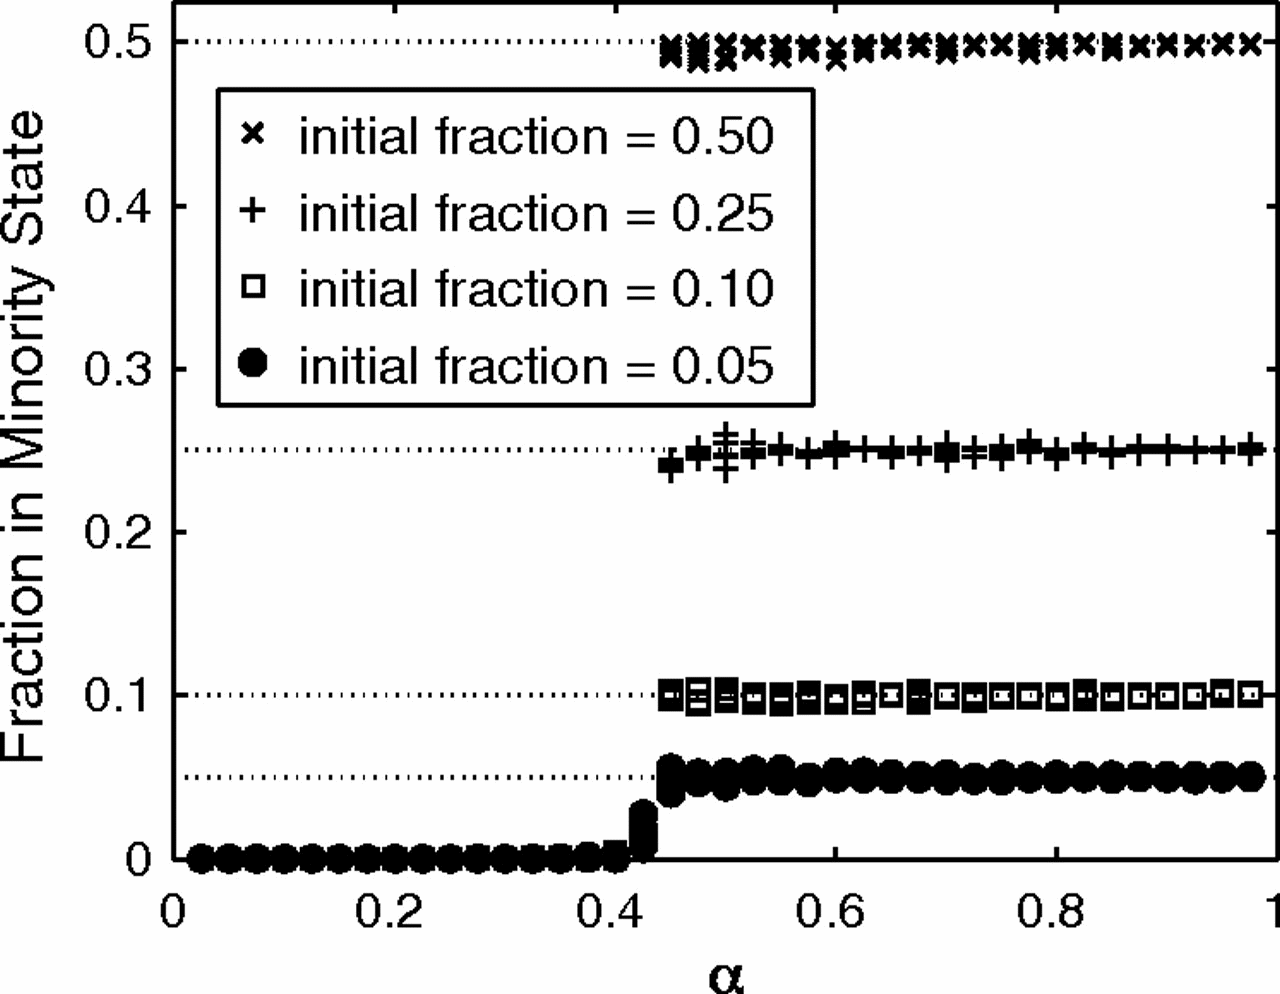
\includegraphics[height=65mm]{rwToSameBifDiag}
  \caption{Final minority fraction as a function of $\alpha$ and initial minority fraction (rewire-to-same), taken from \cite{durret:pnas12}.}
  \label{fig:durretRWtoSameBD}
\end{figure}

\begin{figure}
  \centering
  \subfloat[Only includes runs that have reached consensus]{
    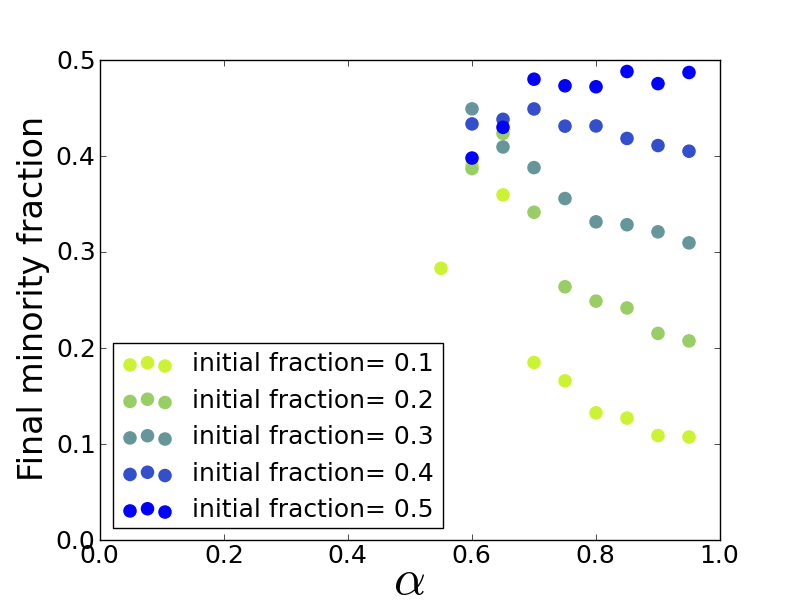
\includegraphics[width=72mm]{bifData_same_1000_4}
    \label{fig:rwSameA}
  }
  \hspace{3mm}
  \subfloat[Includes all runs, even if conflicts exist at the simulation's end] {
    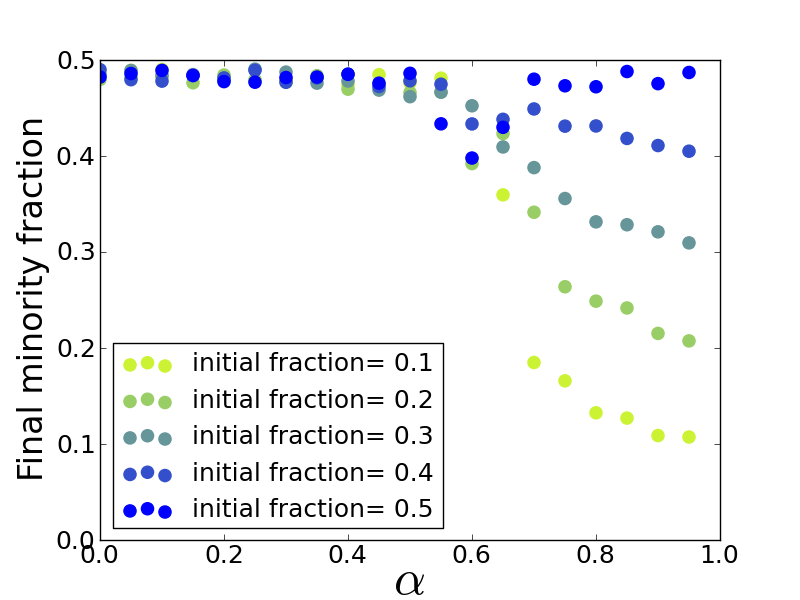
\includegraphics[width=72mm]{bifData_noConvergence_same_1000_4}
    \label{fig:rwSameB}
  }
  \caption{Same data as Fig. \ref{fig:durretRWtoSameBD}, taken from our implementation}
  \label{fig:myRWtoSameBD}
\end{figure}

Figs. \ref{fig:durretRWtoSameBD} and \ref{fig:myRWtoSameBD} reveal differences even in the rewire-to-same variant. While for large $\alpha$ the two appear to agree, our diagram appears to show the curves sloping towards one another, before failing to converge in the allowed number of iterations. Fig. \ref{fig:rwSameB} suggests that a bifurcation occurs as $\alpha$ is decreased, after which the system fluctuates around a minority fraction of 0.50 regardless of $\alpha$ or initial conditions.

\begin{figure}
  \centering
  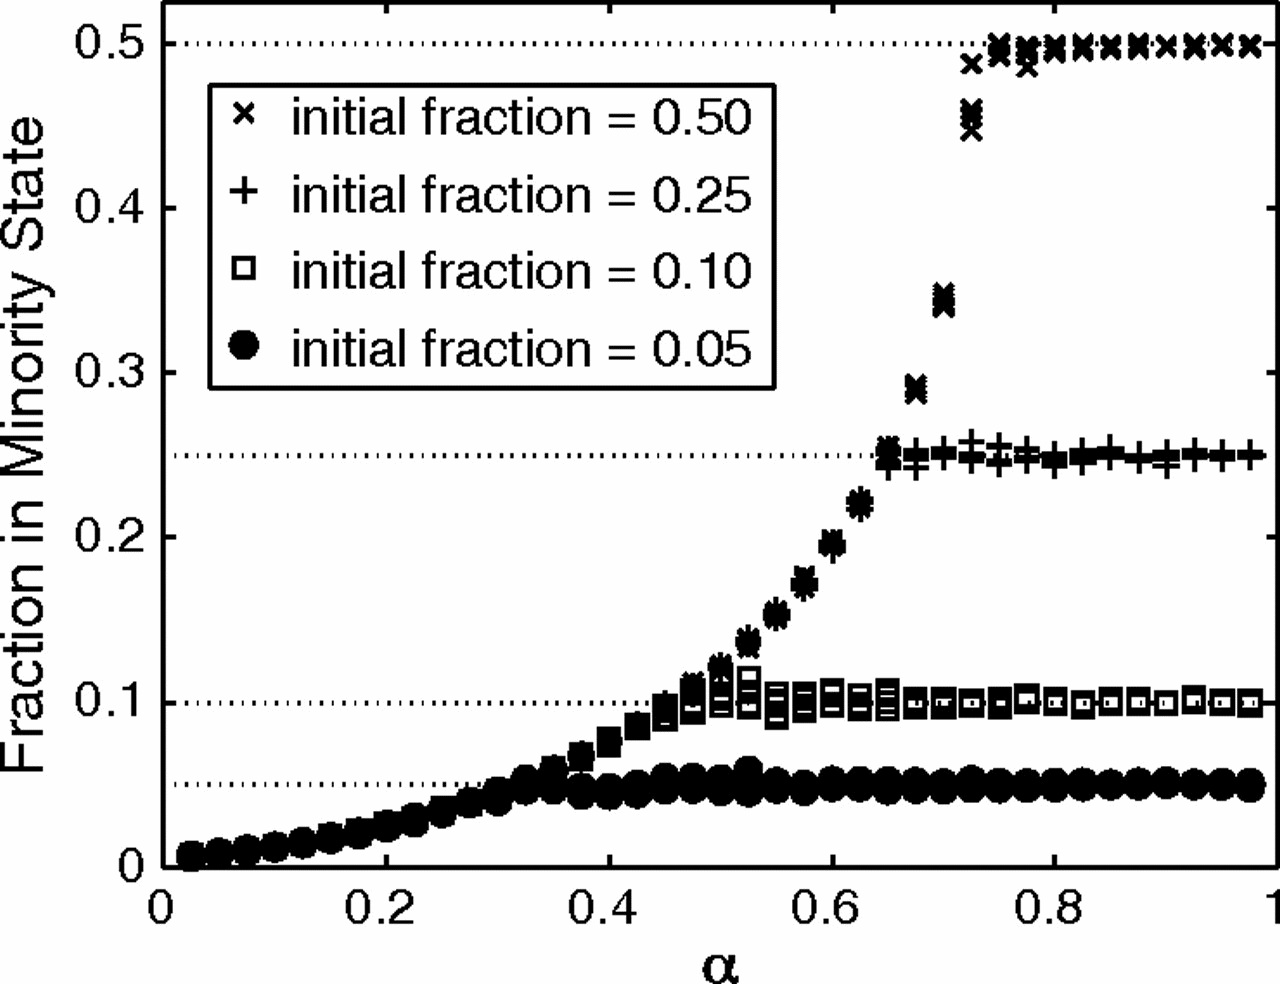
\includegraphics[height=65mm]{rwToRandomBifDiag}
  \caption{Final minority fraction as a function of $\alpha$ and initial minority fraction (rewire-to-random), taken from \cite{durret:pnas12}.}
  \label{fig:durretRWtoRandomBD}
\end{figure}

\begin{figure}
  \centering
  \subfloat[Runs that reached consensus]{
    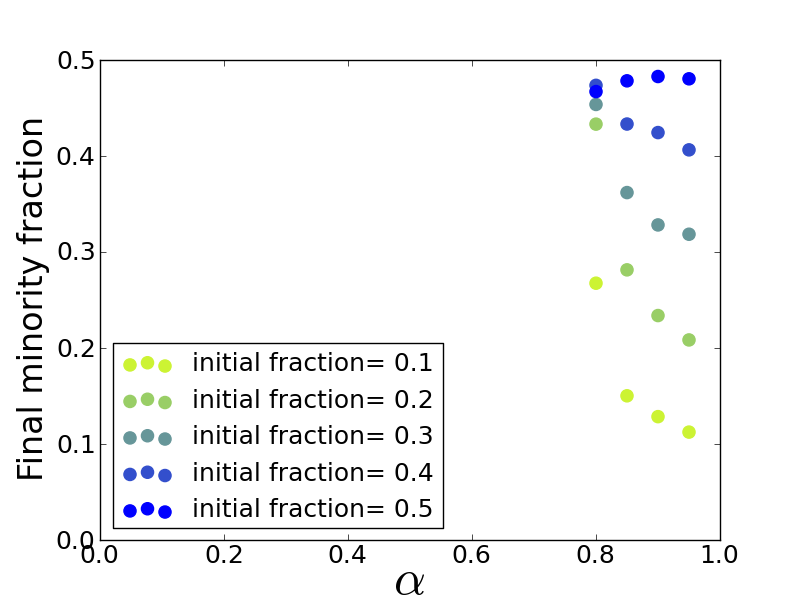
\includegraphics[width=72mm]{bifData_randomIneqJ_1000_4}
  }
  \hspace{3mm}
  \subfloat[All runs] {
    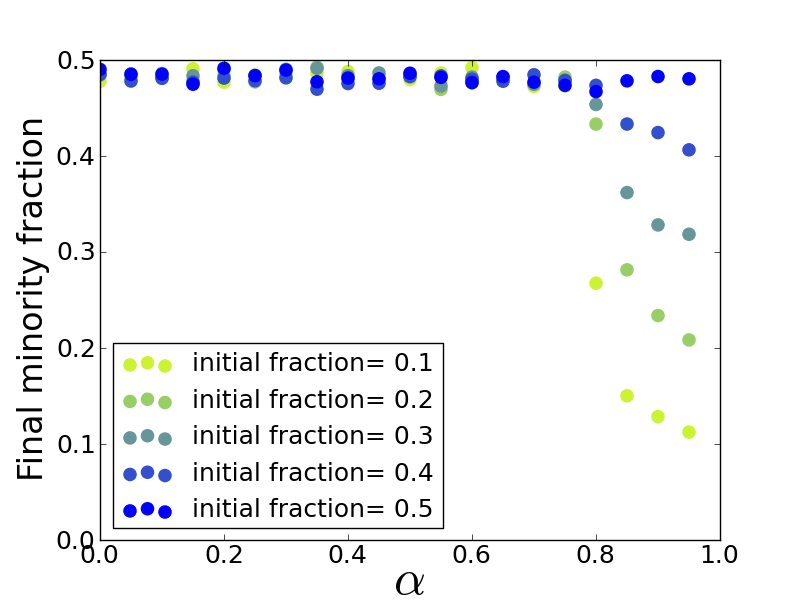
\includegraphics[width=72mm]{bifData_noConvergence_randomIneqJ_1000_4}
    \label{fig:myRWtoRandomFromDiffBDB}
  }
  \caption{Data corresponding to Fig. \ref{fig:durretRWtoRandomBD} from our implementation. In these simulations edges $e_{ij}$ were chosen so that $\xi_{i} \neq \xi_{j}$.}
  \label{fig:myRWtoRandomFromDiffBD}
\end{figure}

\begin{figure}
  \centering
  \subfloat[Runs that reached consensus]{
    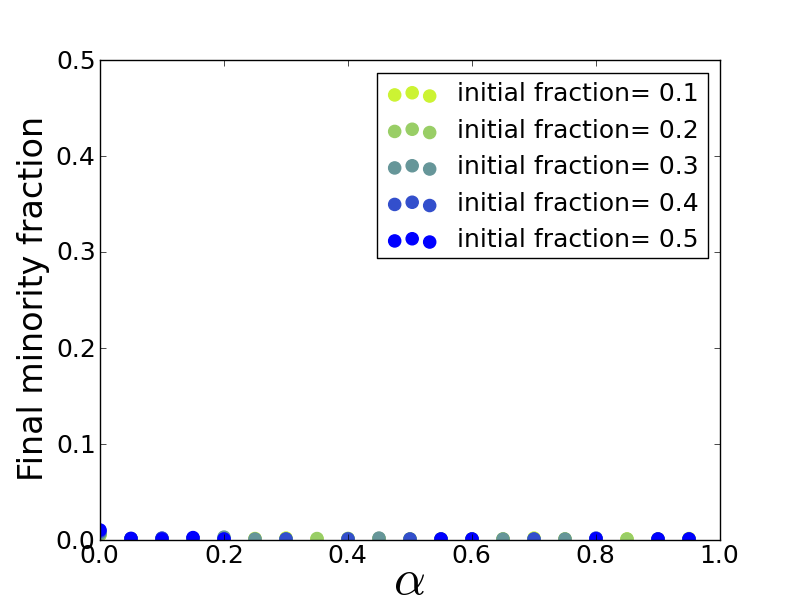
\includegraphics[width=72mm]{bifData_randomIeqJ_1000_4}
  }
  \hspace{3mm}
  \subfloat[All runs] {
    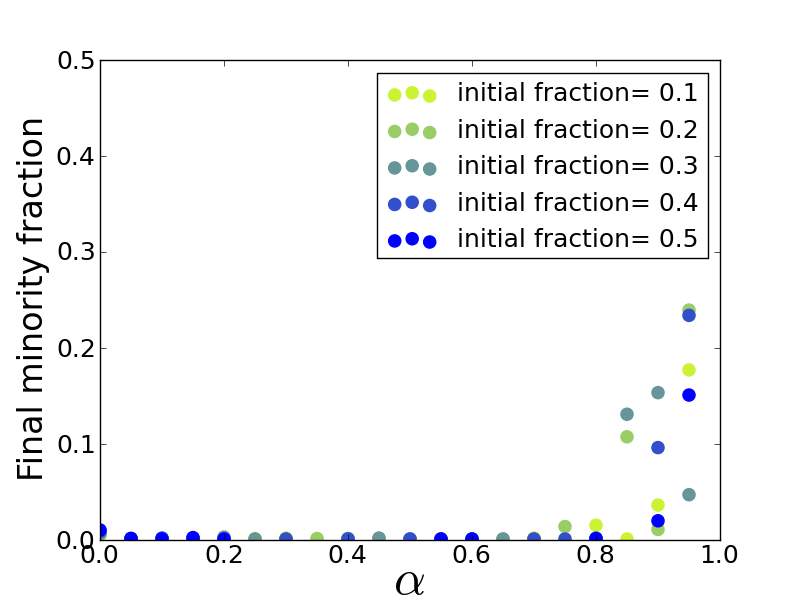
\includegraphics[width=72mm]{bifData_noConvergence_randomIeqJ_1000_4}
    \label{fig:myRWtoRandomFromAllBDB}
  }
  \caption{Data corresponding to Fig. \ref{fig:durretRWtoRandomBD} from our implementation. In these simulations edges $e_{ij}$ were chosen from $V(G)$.}
  \label{fig:myRWtoRandomFromAllBD}
\end{figure}

While certain similarities could be seen between Figs. \ref{fig:durretRWtoSameBD} and \ref{fig:myRWtoSameBD}, it is more difficult to compare the rewire-to-random diagrams, shown in Figs. \ref{fig:durretRWtoRandomBD}-\ref{fig:myRWtoRandomFromAllBD}. Unfortunately, our implementation couldn't recreate the $\alpha_{c}(u_{0})$ curve, and again ran into significant difficulties reaching a consensus state for many values of $\alpha$. From-different simulations again show sloping curves that eventually level off to fluctuate around 0.5. The from-all runs in Fig. \ref{fig:myRWtoRandomFromAllBD} converge to states in which the entire graph shares the same opinion. The few simulations that failed to converge, shown in Fig. \ref{fig:myRWtoRandomFromAllBDB}, almost certainly would've evolved to a single-opinion state if given more time.


\begin{figure}
  \centering
  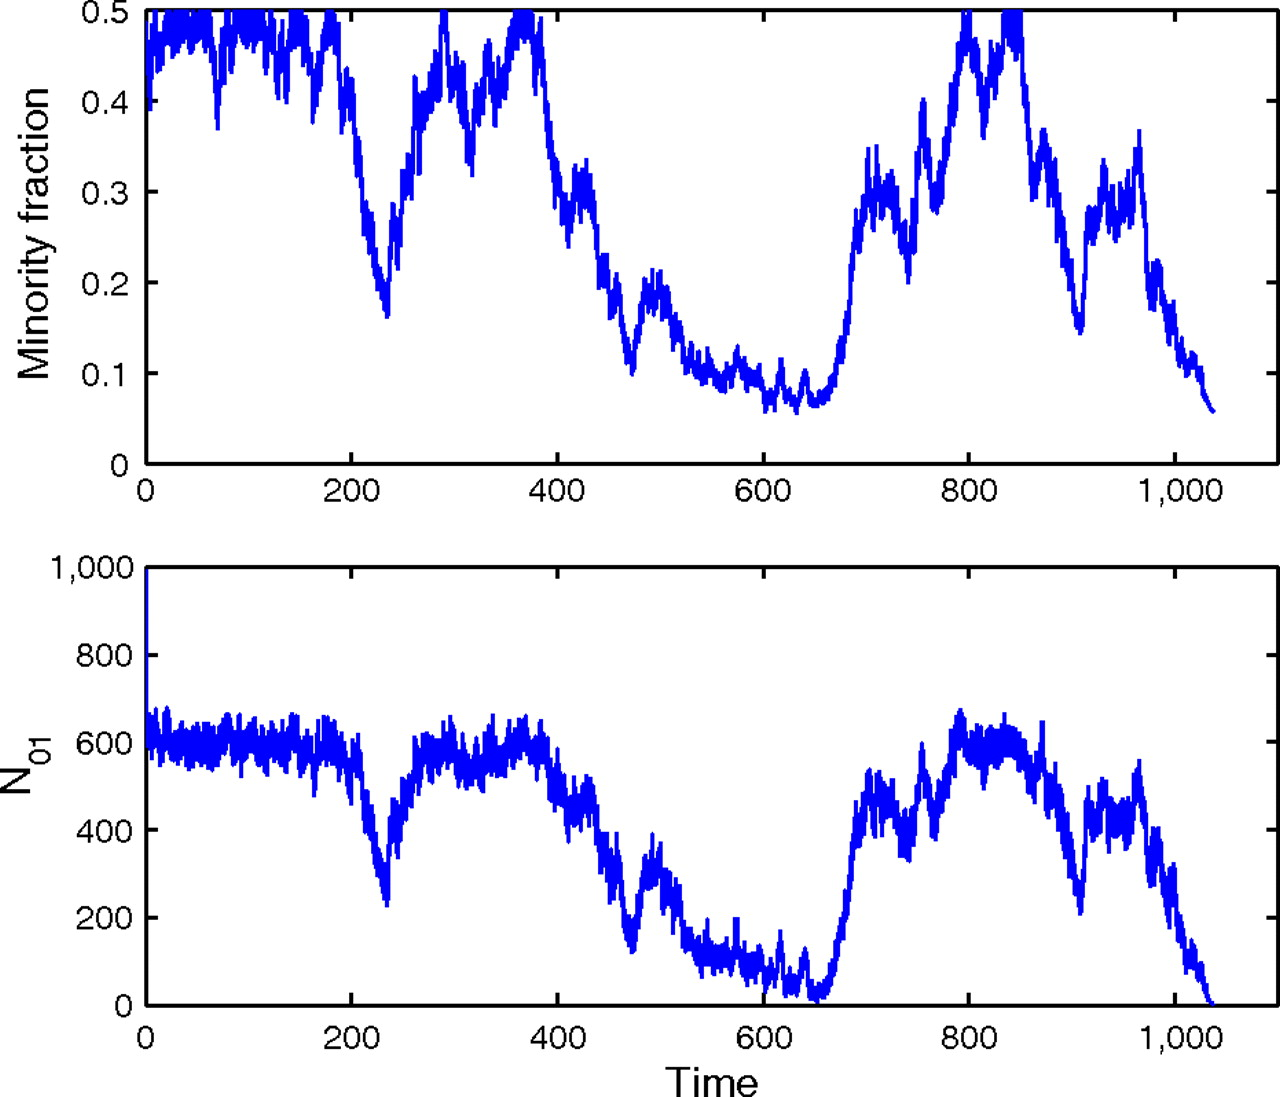
\includegraphics[height=65mm]{durretTimeCourses}
  \caption{Evolution of conflicting edges and minority fraction, taken from \cite{durret:pnas12}.}
  \label{fig:durretTimeCourses}
\end{figure}

\begin{figure}
  \centering
  \subfloat[Runs that failed to reach consensus, $\alpha=0.5$.]{
    \includegraphics[width=72mm]{{graphStats_randomIneqJ_1000_4_0.5_0.5_0.5_noConsensus}.png}
    \label{fig:myIneqJTCsA}
  }
  \hspace{3mm}
  \subfloat[Run that reached consensus, $\alpha=0.8$.] {
    \includegraphics[width=72mm]{{graphStats_randomIneqJ_1000_4_0.8_0.5_0.5_consensus}.png}
  }
  \caption{Evolution of conflicting edges in rewire-to-same, from-different.}
  \label{fig:myIneqJTCs}
\end{figure}

\begin{figure}[h!]
  \centering
  \includegraphics[height=65mm]{{graphStats_randomIeqJ_1000_4_0.5_0.5_0.5_consensus}.png}
  \caption{Evolution of conflicting edges in rewire-to-same, from-all.}
  \label{fig:myIeqJTC}
\end{figure}

We now examine differences in the evolution of individual simulations. Again, the from-different model fails to match the results of \cite{durret:pnas12}. Fig. \ref{fig:myIneqJTCs} reveals that, even when the simulation reaches consensus, the relationship between $N_{01}$ and the minority fraction appears broken, each quantity seems to vary independently of the other. If consensus is not reached, Fig. \ref{fig:myIneqJTCsA} shows that the conflicts and minority opinion oscillate tightly around a well-defined mean. From-all runs recover the covariance, although, as seen in Fig. \ref{fig:myRWtoRandomFromAllBD}, a two-opnion consesnsus is never reached.

\begin{figure}
  \centering
  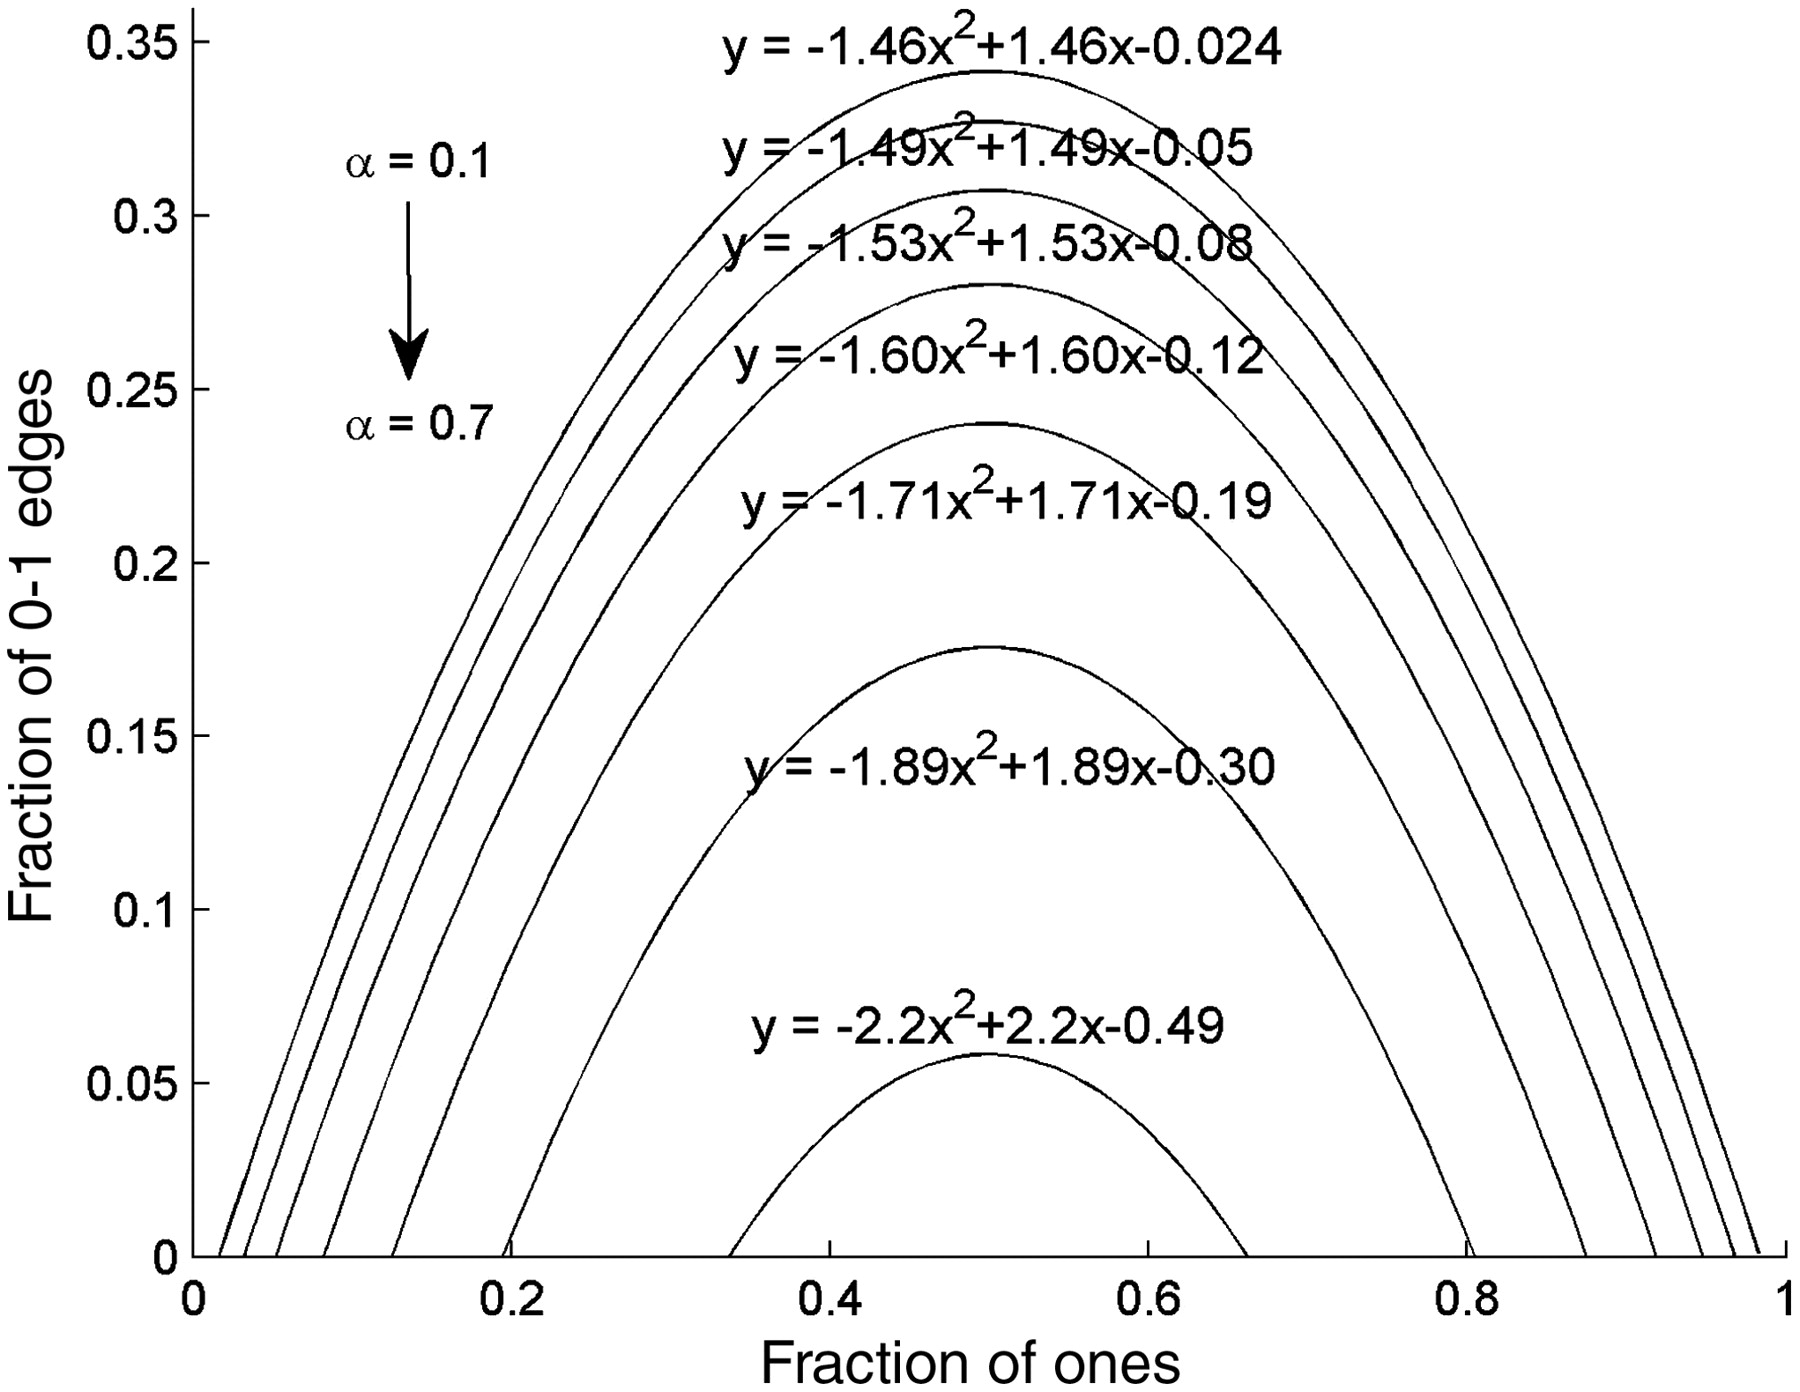
\includegraphics[height=65mm]{durretArcs}
  \caption{Random walk arcs as a function of $\alpha$, from \cite{durret:pnas12}}
  \label{fig:durretArcs}
\end{figure}

\begin{figure}
  \centering
  \subfloat[$e_{ij}\in \{e \in E(G) \mid \xi_{i} \neq \xi_{j}\}$]{
    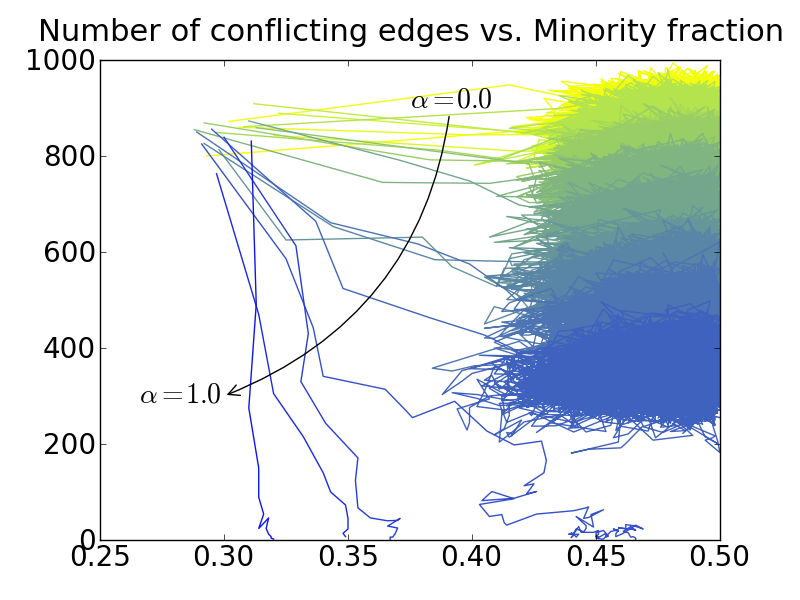
\includegraphics[width=72mm]{nData_randomIneqJ}
    \label{fig:myArcsA}
  }
  \hspace{3mm}
  \subfloat[$e_{ij}\in E(G)$] {
    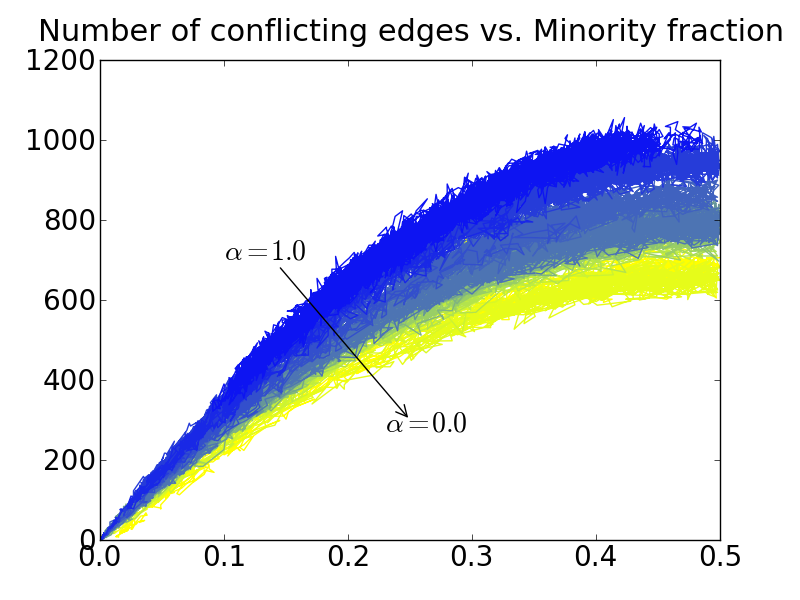
\includegraphics[width=72mm]{nData_randomIeqJ}
  }
  \caption{Random walk arcs from the two different implementations.}
  \label{fig:myArcs}
\end{figure}

Finally, we look at the effects of $\alpha$ on the support interval for the random walk arcs (when present). Fig. \ref{fig:myArcsA} illustrates again the bifurcation in the from-different model. At low $\alpha$, the system doesn't reach consensus, and is trapped around a minority fraction 0.5 and some $N_{01}$. Otherwise, in from-all, random walk behavior is observed, but support is found on (0,1) regardless of $\alpha$'s value, and the overall trend is, in fact, reverse that exhibited in Fig. \ref{fig:durretArcs} (i.e. our curves are flattened as $\alpha$ decreases).\\
The discrepancies displayed above defy obvious explanation, outside of the possibility that our implementation isn't true to the rewire-to-random model described in \cite{durret:pnas12}. However, the system is fairly system, and was straightforward to program. Nonetheless, if the figures above reveal anything, it is that very small changes to the underlying model drastically affect the resultant dynamics. It is worth noting that many of the figures from \cite{durret:pnas12} were from simulations of $n=10,000$ vertices, while ours set $n=1,000$. It would seem this shouldn't have a significant effect on system dynamics; however, this appears to be the only certain difference between the two versions.

\section*{Future work}
Besides having others proof-read our code, we should also try to recreate the figures in \cite{vazquez:prl08}. Even if these, too, disagree, it may offer some insight into the underlying differences.

\bibliographystyle{abbrv}
\bibliography{votingBib}
\end{document}
